\section{Seeking cascade decays}
 
The work in the section was produced in collaboration with Billy Ford, Shubhani Jain, Amit Chakraborty, Stefano Moretti, Emmanuel Olaiya, Claire Shepherd-Themistocleous and Srinandan Dasmahapatra~\cite{chakraborty2020revisiting}.
Working with various established jet clustering techniques the objective was to determine what experimental particle and jet cuts would be needed to observe cascade decays involving light Higgs.
My contribution to this was in developing alternative event processing and jet clustering tools that
validated the results obtained from the standard libraries and allowed in depth inspection of points of confusion.

Remaining in the 2HDM, as in the previous section, we consider an alternative scenario involving a light Higgs.
The heavier CP-even Higgs (\(H\)) is considered to be a SM Higgs at \(125\)GeV,
then should the light CP-even Higgs be \(< 60\)GeV the \(H\rightarrow{} hh\) decay is resonant.
As with the SM Higgs the dominant decay mode for the light Higgs is bottom-antibottom quark pairs~\cite{Moretti1994belowThreshold,Djouadi1995twoAndthree}, so that the predominant final state of \(H\rightarrow{} hh\) is four (anti)quarks\footnote{Notice that the same argument can be made for the case of $gg\to h\to AA\to b\bar b b\bar b$ when $m_A<m_H/2$.}.
Detecting this signal would require identifying these four \bthing{quarks} by clustering their decay products into jets.
Various algorithms are establish for jet clustering, here, both the popular
anti-kt~\cite{Cacciari2008akt} and Cambridge-Aachen algorithms~\cite{Wobisch1998caJet} and the
more recent variable-\stoppingdeltar{} method~\cite{Krohn2009variableR}. 
We will investigate whether such variable-\stoppingdeltar{} jets can improve the ability to observe particular 2HDM-II four \bthing{jet} final state topologies. 

\subsection{Monte Carlo and tagging}\label{sec:dataset6040}

We consider two sample benchmark points, namely, $m_{h}$ = 40 GeV and 60 GeV, while  fixing $m_{H}$ = 125 GeV, within a 2HDM Type-II (2HDM-II henceforth), which have been tested against theoretical and experimental constraints by
using 2HDMC \cite{Eriksson20102HDMC}, HiggsBounds \cite{Bechtle2014higgsbounds4}, HiggsSignals \cite{Bechtle2014higgssignals} as well as checking flavour constraints with SuperISO \cite{Mahmoudi2008SuperIso}. 
Using Madgraph~\cite{alwall_madgraph2011} to generate the partonic process, and Pythia~\cite{sjostrand_pythia2015} to shower, ${\cal O}(10^5)$ of \(pp \rightarrow{} H \rightarrow{} hh \rightarrow{} b\bar{b}b\bar{b}\) events are generated, with $\sqrt{s}=13 $ TeV.

To label a jet as a \bthing{jet} Monte Carlo (MC) information is used.
The \bthing{quarks} that we aim to capture in jets are identified and
assigned to the closest jet in angular (\distancedeltar{}) distance
unless the closest jet is further away than the cut off parameter \stoppingdeltar{},
in which case the quark is abandoned.
To mimic a more realistic tagging efficiency a
\(25\%\) false negative rate is added to this,
and a \(10\%\) false positive rate, in the form of \(c\)-quark
jets appearing as \bthing{jets}, is applied to this selection.

\subsection{Cutflow}\label{sec:cutflow}

Typical cuts used for Higgs decay chains,
such as those seen in~\cite{Sirunyan2018alljet},
tend to be restrictive with the objective of 
ensuing fully hadronic signature. 
In this example the cuts given are;
\begin{enumerate}
    \item Remove all final state particles with a $p_T < 0.5$ GeV and $|\eta| > 2.5$.
    \item Perform jet reconstruction and $b$-tagging in \fastjet{} \cite{Cacciari2011FastJet}, with specified clustering algorithm and \stoppingdeltar{}.
    \item Remove $b$-jets with $p_T < 30$ GeV $(*)$.
    \item Remove $b$-jets whose energy content due to electrons(muons) is greater than  90(80)\%.
    \item Remove $b$-jets whose energy content due to neutral hadrons and photons is greater than 90\%.
    \item Remove $b$-jets with zero charged hadron energy.
    \item Remove $b$-jets with only one constituent.
\end{enumerate}

For the process considered here, 
these cuts remove the vast majority of the signal.
Taking a \(p_T < 30\)GeV cut on the jet culls many events,
see figure~\ref{fig:bjetpt}.
A more permissive set of jet cuts is seen in~\cite{Sirunyan2019exotic}.
In~\cite{Sirunyan2019exotic} $p_T$ of the leading $b$-jet is required to have $>20$GeV, and others $p_T > 15$GeV. 
 This reduced cutflow would require the implementation of a trigger with $p_T$ thresholds of 15, 10, 10, 10GeV for the four ($p_T$ ordered) $b$-jets.
 These $p_T$ thresholds are sufficiently below our jet $p_T$ requirement to enable $100\%$ efficiency in the trigger. 

A comparison of the \bthing{jet} multiplicity of events with
typical cuts, permissive cuts and no cuts can be seen in~\ref{fig:nbjets}.
\begin{figure}[htb!]
	\centering
	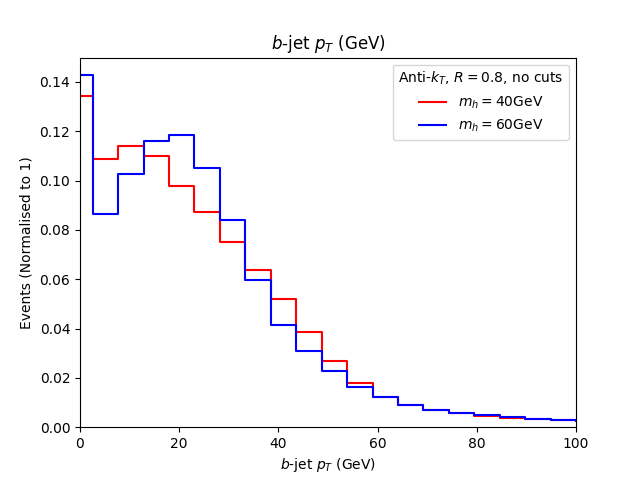
\includegraphics[scale=0.6]{plots/bjetpt_AK8_nocuts.png}
    \caption{Transverse momentum distribution of all $b$-jets with no cuts imposed on the jets or on the final state hadrons. We have used here $\stoppingdeltar{}=0.8$, though the pattern is similar for $\stoppingdeltar{}=0.4$. Here, we have used the anti-$k_T$ jet clustering algorithm.}
\label{fig:bjetpt}
\end{figure}
as can be seen with the comparison given in figure~\ref{fig:nbjets}.
\begin{figure}[t!]
	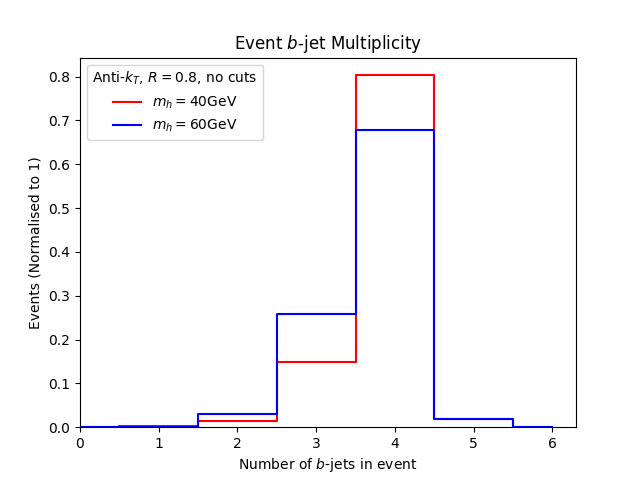
\includegraphics[scale=0.5]{plots/nbjets_AK8_nocuts.png}
	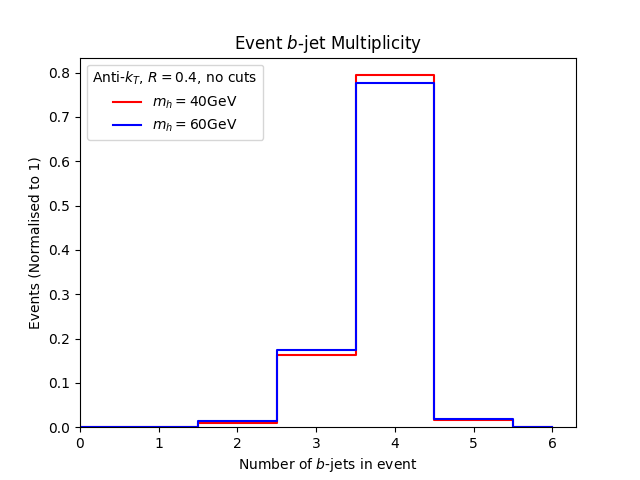
\includegraphics[scale=0.5]{plots/nbjets_AK4_nocuts.png}
	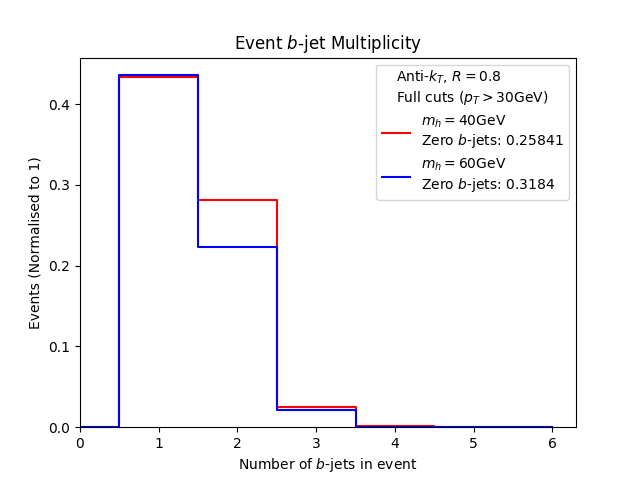
\includegraphics[scale=0.5]{plots/nbjets_AK8_pt30.png}
	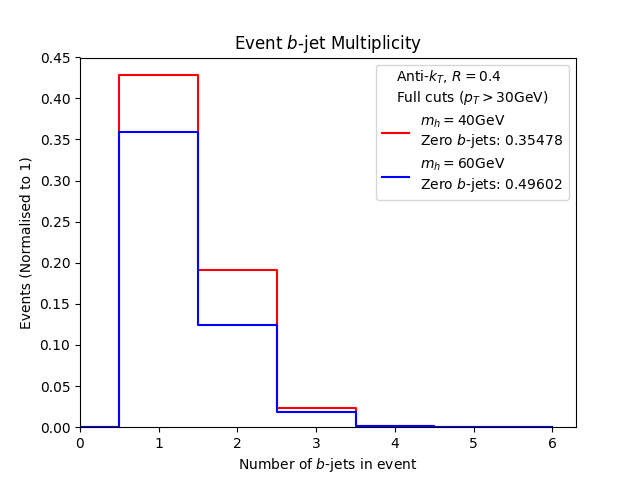
\includegraphics[scale=0.5]{plots/nbjets_AK4_pt30.png}
	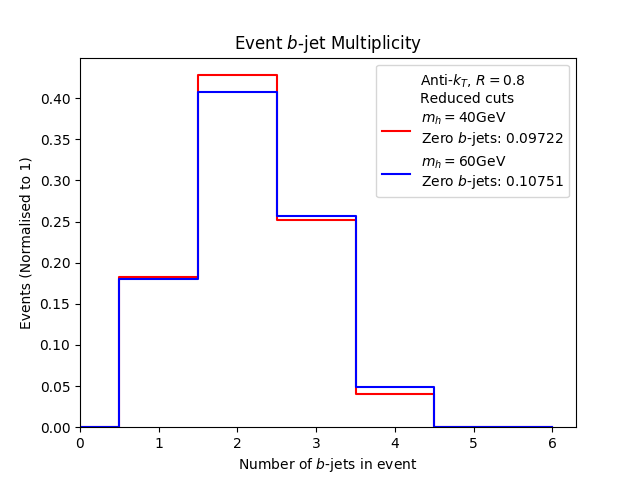
\includegraphics[scale=0.5]{plots/nbjets_AK8_lowptcut.png}
	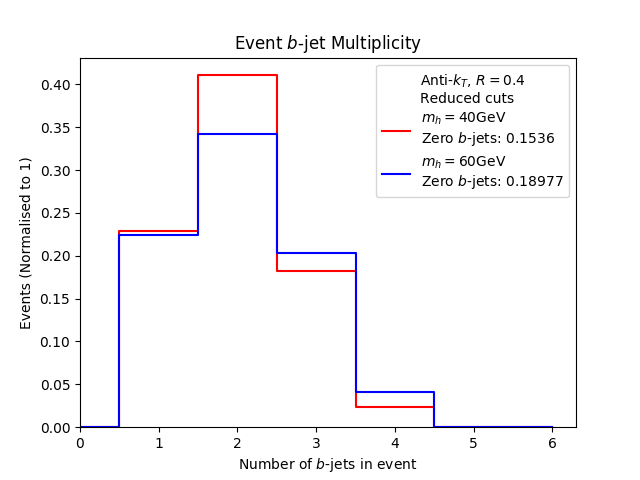
\includegraphics[scale=0.5]{plots/nbjets_AK4_lowptcut.png}\\
	\caption{The distributions of $b$-jet multiplicities under various cutflows.
        The left column presents anti-kt jets where \(\stoppingdeltar{}=0.8\) and the right column has \(\stoppingdeltar{}=0.4\).
        The first row is the distribution with no cuts on the inputs or the jets,
        the second row shows the impact of typical cuts (as described in sec~\ref{sec:cutflow}),
        the third row shows the results of the possible relaxation (suggested in sec~\ref{sec:cutflow}).
        Note that events containing zero $b$-jets are not plotted but included in the legend, in the case of no cuts being applied all events contain at least one $b$-jet.}
\label{fig:nbjets}
\end{figure}

From this point on the permissive cuts will be employed as they seem necessary
for an attempt to retain this signal.

\subsection{Variable-\stoppingdeltar{} clustering}
The standard jet clustering algorithms, anti-kt and Cambridge-Aachen,
both depend on a interparticle distance,
\( d_{ij} = \text{min}(p^n_{Ti}, p^n_{Tj})\distancedeltar{}^2_{ij}\), 
and a beam distance,
\( d_{Bi} = p^n_{Ti}\distancedeltar{}^2\).
The algorithm is agglomerative, to begin 
all interparticle distances and beam distances are calculated,
the smallest value is found.
If the smallest value is an interparticle distance 
then those particles are combined,
otherwise, if the smallest value is a beam distance
then the corresponding particle is deemed a complete jet and removed.
This process repeats until all particles are removed.

The variable-\stoppingdeltar{} determines how far from it's nearest neighbour
a combined particle must be such that it is removed and deemed a jet.

Variable-\stoppingdeltar{} is a slight divergence from this that allows the
value of \stoppingdeltar{} to change with the \(p_T\) of the particle.
\stoppingdeltar{} becomes \(\stoppingdeltar{}_\text{eff}(p_T) = \frac{\rho}{p_T}\), where \(\rho\)
is a tunable parameter.

\begin{figure}[htb!]
	\begin{center}
	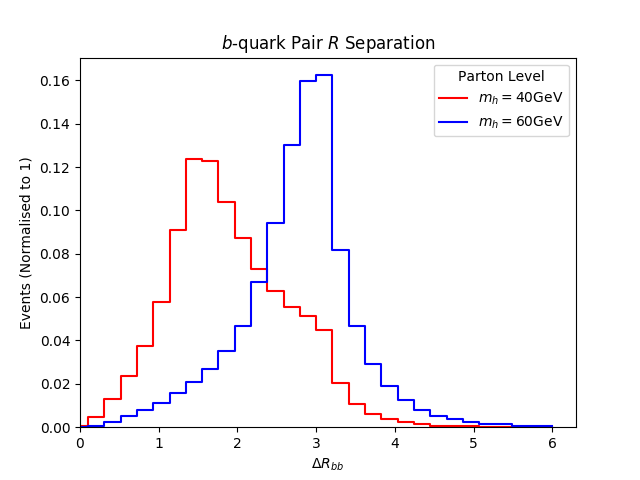
\includegraphics[scale=0.42]{plots/parton/delRbb.png}
	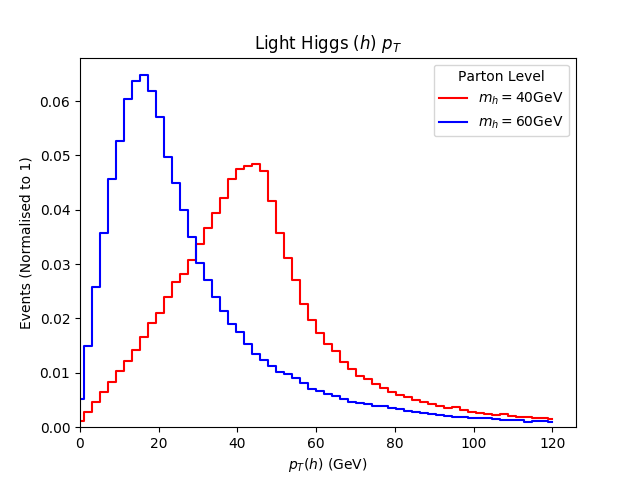
\includegraphics[scale=0.42]{plots/parton/LHiggs_pt.png}
	 \end{center}
     \caption{Left: the \distancedeltar{} distribution between the
two $b$-partons originating from the same $h$.
Right: the $p_T$ distribution of the light Higgs boson $h$ originating from $H$ decay.
No (parton level) cuts have been enforced here. }
\label{fig:parton_higgs}
\end{figure}

An indication of why this might be desirable can be seen by
looking at the angular separation of \bthing{quarks} originating from the 
same \(h\), seen in figure~\ref{fig:parton_higgs}.
There is a considerable range of angular separations for each decay,
in general, the angular separation between the decay products $a$ and $b$  in the resonant process
$X \to a b$ can be approximated as $\distancedeltar{} (a,b) \sim \frac{2 m_{X}}{p^{X}_T}$.

Indeed the variable-\stoppingdeltar{} algorithm does produce notably sharper mass peaks,
as can be seen in figure~\ref{fig:invmass2}.

\begin{figure}[htb!]
	%\centering
	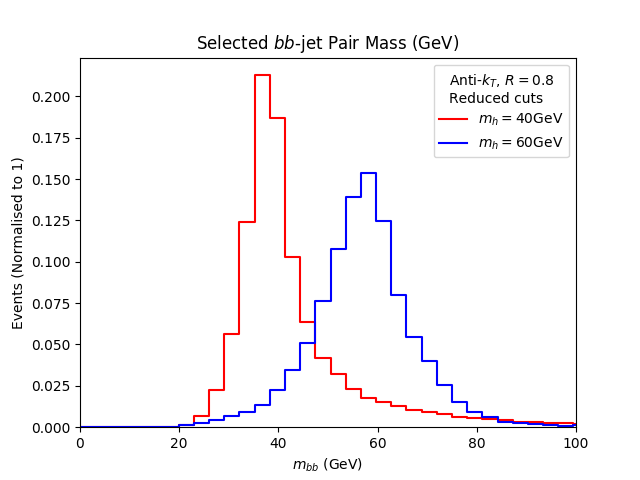
\includegraphics[scale=0.5]{plots/bbmass_AK8_lowptcut.png}
	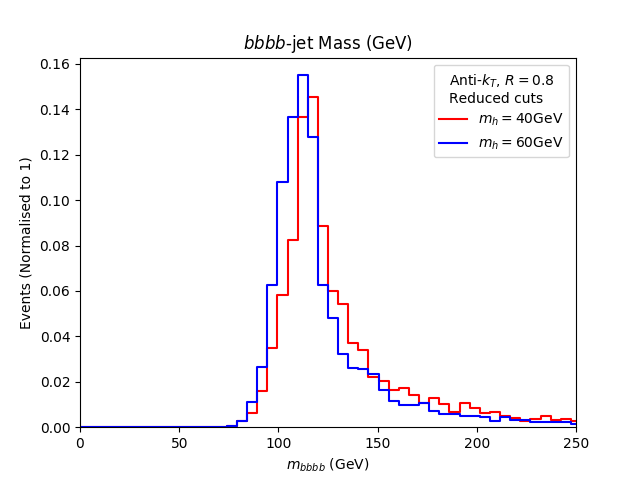
\includegraphics[scale=0.5]{plots/bbbbmass_AK8_lowptcut.png}
	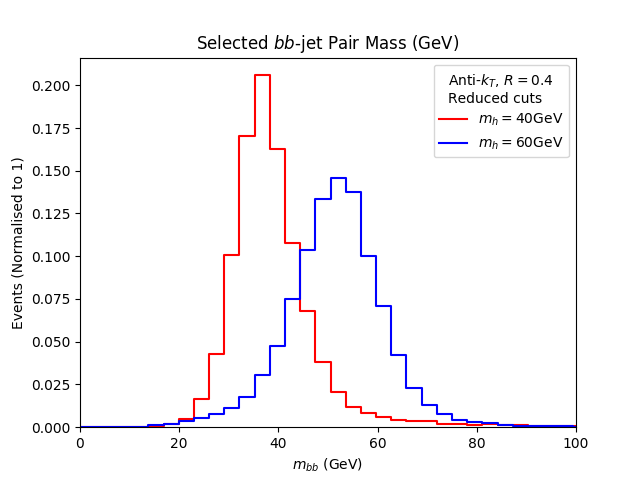
\includegraphics[scale=0.5]{plots/bbmass_AK4_lowptcut.png}
	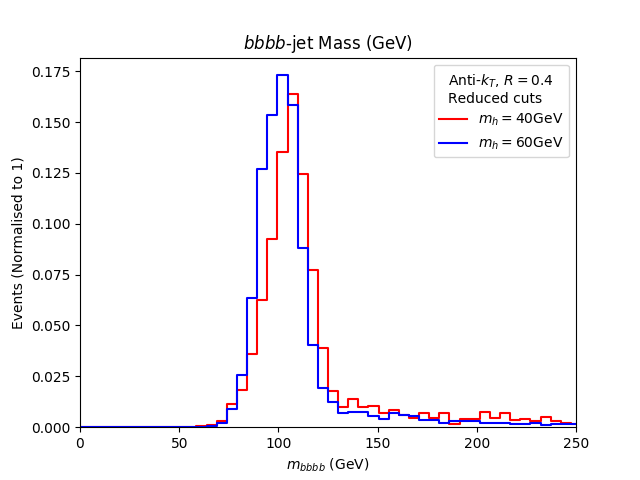
\includegraphics[scale=0.5]{plots/bbbbmass_AK4_lowptcut.png}
	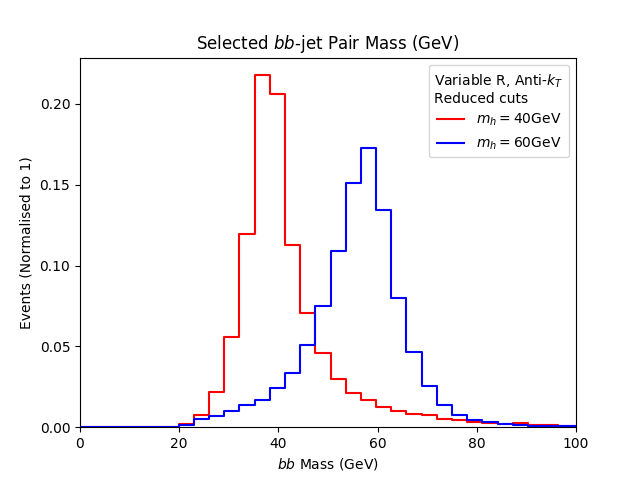
\includegraphics[scale=0.5]{plots/bbmass_varR_lowptcut.png}
	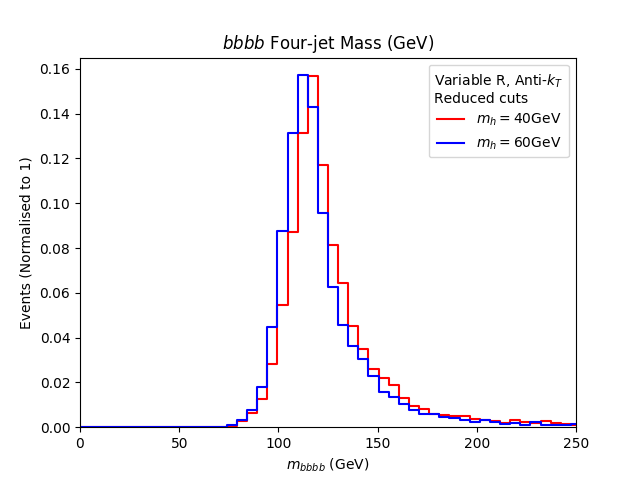
\includegraphics[scale=0.5]{plots/bbbbmass_varR_lowptcut.png}
	\caption{The distributions in invariant mass of two (left panels) and four (right panels) $b$-tagged jets, in presence of the
  reduced $p_T$ cuts on the $b$-jets.
  The first two rows are anti-kt clusterings, with \stoppingdeltar{} equal to \(0.8\) and \(0.4\) respectively,
  The final row shows the variable-\stoppingdeltar{} algorithm.}
\label{fig:invmass2}
\end{figure}


To quantify this improvement the significance of the signal over the background is calculated for two values of (integrated)  luminosity, e.g.,  ${\mathcal{L}}=$  140 and 300 fb$^{-1}$.
The event rate ($N$) for the various processes is given by:
%
\begin{equation}
N \ = \sigma \times \mathcal{L}.
\end{equation}
%
With these event rates, the significance, $\Sigma$, is given by;
%
\begin{equation}
\Sigma = \frac{N(S)}{\sqrt{N(B_{b\bar{b}b\bar{b}})+N(B_{Zb\bar{b}})+N(B_{t\bar{t}})}}.
\end{equation}
%
The results of this are shown in tables.~\ref{tab:signalbackground4}--\ref{tab:signalbackground5}.
It is clear that that the variable-\stoppingdeltar{} approach works better than the fixed-\stoppingdeltar{} one also in providing the best significances, no matter the choices of \stoppingdeltar{} for the latter.  The improvement in the final significances is indeed very significant.



\begin{table}[!h]
\begin{center}
\scalebox{0.8}{
\begin{tabular}{ |c|c|c|c| }
 \hline
 & Var-\stoppingdeltar{}, $\rho=20$ GeV  & $\stoppingdeltar{}=0.4$ & $\stoppingdeltar{}=0.8$    \\
 \hline
$40~\text{GeV}$ &0.358 & 0.061 & 0.160 \\
 \hline
$60~\text{GeV}$ & 6.677&2.074 & 3.138  \\
\hline
\end{tabular}
}
\caption{\label{tab:signalbackground4} Final $\Sigma$ values calculated for signal and backgrounds for ${\cal L}=140$ fb$^{-1}$  upon enforcing the reduced cuts plus the mass selection criteria $|m_{bbbb}-m_H|< 20$ GeV and $|m_{bb} - m_h|< 15$ GeV for the various jet reconstruction procedures.}
\end{center}
\end{table}

\begin{table}[!h]
\begin{center}
\scalebox{0.8}{
\begin{tabular}{ |c|c|c|c| }
 \hline
 & Var-\stoppingdeltar{}, $\rho=20$ GeV  & $\stoppingdeltar{}=0.4$ & $\stoppingdeltar{}=0.8$    \\
 \hline
$40~\text{GeV}$ & 0.524 & 0.089 & 0.234 \\
 \hline
$60~\text{GeV}$  & 9.775 &3.036  & 4.594  \\
\hline
\end{tabular}
}
\caption{\label{tab:signalbackground5} Final $\Sigma$ values calculated for signal and backgrounds for ${\cal L}=300$ fb$^{-1}$  upon enforcing the reduced cuts plus the mass selection criteria $|m_{bbbb}-m_H|< 20$ GeV and $|m_{bb} - m_h|< 15$ GeV for the various jet reconstruction procedures.}
\end{center}
\end{table}

\subsection{Conclusions}
In this paper, we have assessed the potential scope of the LHC
experiments in accessing BSM Higgs signals induced by cascade decays
the following prototypical production and decay channel: $gg\to H\to
hh$, where $H$ is the SM-like Higgs state and $h$ is a lighter BSM
Higgs state.
The latter is extremely difficult to establish at the LHC,
owing to the substantial hadronic background.

The first message we deliver is that, with current $p_T$ limitations on final state $b$-jets, using a fixed-\stoppingdeltar{} jet reconstruction and tagging procedure will lead to a poor signal visibility, with a majority of signal $b$-jets being lost. We present a reduced cut flow, based on existing $b\bar b\mu^+\mu^-$ analyses, and show that this indeed provides a window into final states of $gg \rightarrow H \rightarrow hh \rightarrow bb\bar{b}\bar{b}$ decays with $m_H = 125$ GeV and $m_h < \frac{m_H}{2}$. 

Additionally, we test a variable-\stoppingdeltar{} reconstruction approach, and show a significant improvement in signal yield, as well as signal-to-background rates.

